\subsubsection{Address Length Evaluation}\label{sec:address-evaluation}

We now evaluate the address generation schemes in terms of address length. The
common component in all address cases is the hash value of the verification
payment key $\paymentkeyverify$, which is the minimum amount of information an
address needs to contain. So far this has been the only component of the
address in blockchain protocols, like Bitcoin. However, for different types of
addresses, the extra information, like the staking object $\beta$, may increase
the length of the address measurably.

We compare addresses in terms of bits, rather than the amount of the address's
characters. Specifically, although addresses are usually encoded in Base58, we
compare the encoded information itself. Therefore, for Bitcoin the address
information is $256$ bits, consisting of the hash of the payment key. Cardano
uses the \texttt{BLAKE2b-224} hash function, so its ``delegated" type of
address is typically $608$ bits long, consisting of the payment key hash ($224$
bits), the staking key hash ($256$ bits) and a searchable tag ($128$ bits).

In the fully malleable scheme of Section~\ref{subsubsec:malleable_addrgen}, all
addresses contain a single extra information component, the staking object
$\beta$. For the base address, $\beta$ is a hash value, similar to the payment
key's, so it is $512$ bits. A pointer comprises of three attributes $ptr = (b,
x, c)$, where $b$ is the block index, $x$ the transaction index and $c$ the
certificate index. Although these parameters are adjustable, it is safe to
assume that $b$ is $30$ bits, since, in a system that produces blocks every
$20$ seconds, $30$ bits are enough to describe blocks for over $700$ years, $x$
is $20$ bits, assuming $1$ million transactions per block, and $c$ is $5$ bits,
constraining the amount of certificates per transaction to $32$. Given these
assumptions, the length of the pointer address is $256 + 30 + 20 + 5 = 311$
bits, which is a notable reduction in the address's size. For exile addresses,
we assume that $\epsilon$ is the empty string. Although this prohibits from
distinguishing between different types of exile addresses, it is a valid
assumption in the cases when we do not need such distinction, but simply remove
their stake from the PoS protocol's execution. Therefore, the length of exile
addresses is $256$ bits. As we see, all addresses in the malleable setting are
shorter than Cardano and slightly longer than or equal to Bitcoin.

In the ``sink" malleable scheme of Section \ref{subsec:nm-genaddr}, the length
of all types of addresses is the sum of our calculations above plus the length
of the signature. The ECDSA signature length is typically equal to $132$ bytes,
hence each type of addresses is $132$ bytes longer compared to the fully
malleable scheme. We see now that ``sink" malleable addresses are much longer,
compared to both Bitcoin and Cardano.

Figure \ref{graph:addr_length} summarizes the above discussion on address
lengths for our address generation schemes.

\begin{figure}
  \begin{center}
    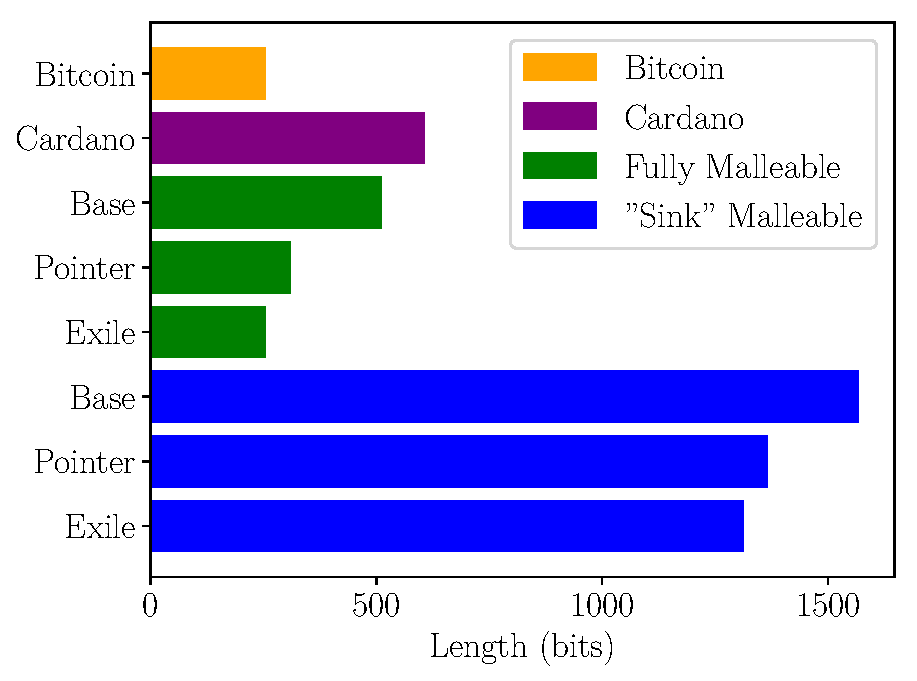
\includegraphics[width=0.7\textwidth]{figures/delegation/address_gen.pdf}
  \end{center}
  \caption{Length comparison of the fully and sink malleable addresses with the
    addresses of Bitcoin and Cardano.}
  \label{graph:addr_length}
\end{figure}

\subsubsection{Wallet Recovery Evaluation}\label{sec:recovery-evaluation}

Recovery should, in principle, be a quick process, since it is an essential
part of the wallet's initialization process. During recovery, the wallet
creates a (sorted) index of all addresses in the ledger, which enables a quick
lookup of addresses, \ie finding the transactions which correspond to a given
address. Naturally, the index creation takes $O(m\log(m))$, where $m$ is the
total number of addresses \emph{in the ledger}. In practice, in order to
enhance performance the index can be retrieved from the network and then only
verified by the wallet. Next, the wallet computes the recovery tags for its
addresses. We assume that unused addresses need not be recovered and are
recomputed upon demand. By using incremental index sets, the asymptotic
complexity of identifying all indexes is $O(n)$, $n$ being the number of
\emph{the wallet's addresses}, thus the complexity of wallet recovery is
$O(n\log(m))$. In our scheme, the recovery tag is the hash of the payment key,
so its computation requires deriving the child payment key and then hashing it.
Although hashing and comparison are simple operations, key derivation includes
elliptic curve point multiplication, which is rather expensive. Our benchmarks,
performed on an Intel Core $i7-6500U$ CPU, show that deriving a single key
requires approximately $23$ms; assuming that a regular user's wallet controls
at most $100$ addresses, identifying all tags requires roughly $2.3$ seconds.
Figure \ref{graph:recovery} depicts the comparison between the recovery scheme
of Section~\ref{subsec:address-attributes} and the searchable recovery scheme
(described in Section~\ref{subsubsec:searchable_tags}) used in existing
systems, like Cardano. The searchable scheme relies on decryption, which is
measured at $1$ms, hence the wallet's recovery requires $10^3$ seconds.
However, the asymptotic complexity is $\Theta(m)$ which, given $m \gg n$, is
worse than our scheme. Here, we set $m = 10^6$, a (very) optimistic estimate in
real world terms; for larger $m$, the performance gap is even more apparent.

\begin{figure}
  \begin{center}
    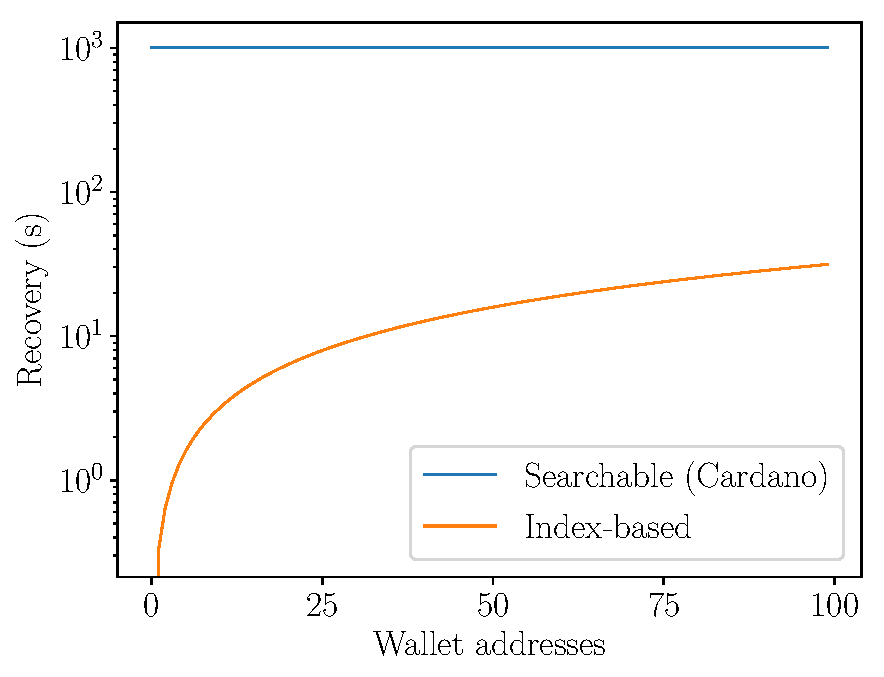
\includegraphics[width=0.7\textwidth]{figures/delegation/recovery.pdf}
  \end{center}
    \caption{Comparison of the index-based recovery scheme and the
    searchable-based scheme employed by Cardano. The asymptotic complexity for
    the searchable scheme is $\Theta(m)$ while for our index scheme is
    $\O(n\log(m))$, $m$ being the number of the entire ledger's addresses (set
    to $10^6$) and $n$ the number of the wallet's addresses (the horizontal
    axis).}
  \label{graph:recovery}
\end{figure}
